% Section: Using Abisko
% Latex file for the MPI Course at HPC2N Umea 
%    Elaborated by P. Ojeda
%

%########################  NEW SECTION  ########################
\section{Linux}

%%%%%%%%%%%%%%%%% NEW  SLIDE
\begin{frame}
	\frametitle{Linux OS}
	
        \begin{center}
        \includegraphics[width=6.0cm]{images/linux_os.png}
        {\small Linux OS components.}
        \end{center}
\end{frame}

%%%%%%%%%%%%%%%%% NEW  SLIDE
\begin{frame}
	\frametitle{Linux }
	\begin{itemize}
		\item	UNIX-like OS 
		\item	used in modern Android smartphones
		\item   the difference between all UNIX-like OS is small	
	\end{itemize}
	
\end{frame}

%%%%%%%%%%%%%%%%%%%%%%%%%%%%%%%%%%%%%%%%%%%%%%%%%%%%%%%%%%%%%%%%%%%%%%%%%%%%%%%%%%%%%
\begin{frame}
	\frametitle{Linux timeline}
        \begin{center}
        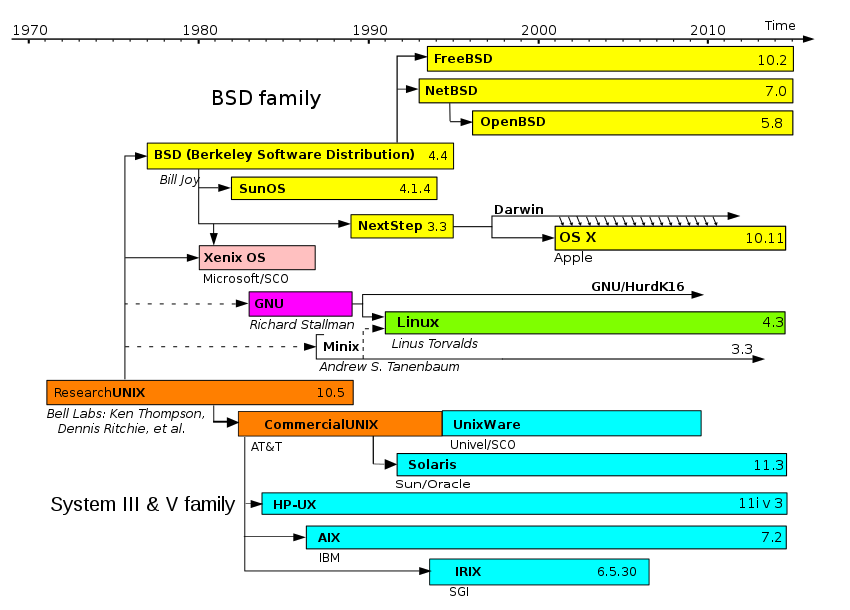
\includegraphics[width=8.0cm]{images/Unix_timeline.png}
        \end{center}
        {\tiny source: wikipedia}
\end{frame}

%%%%%%%%%%%%%%%%%%%%%%%%%%%%%%%%%%%%%%%%%%%%%%%%%%%%%%%%%%%%%%%%%%%%%%%%%%%%%%%%%%%%%
\begin{frame}
	\frametitle{The Linux terminal}
        \begin{center}
        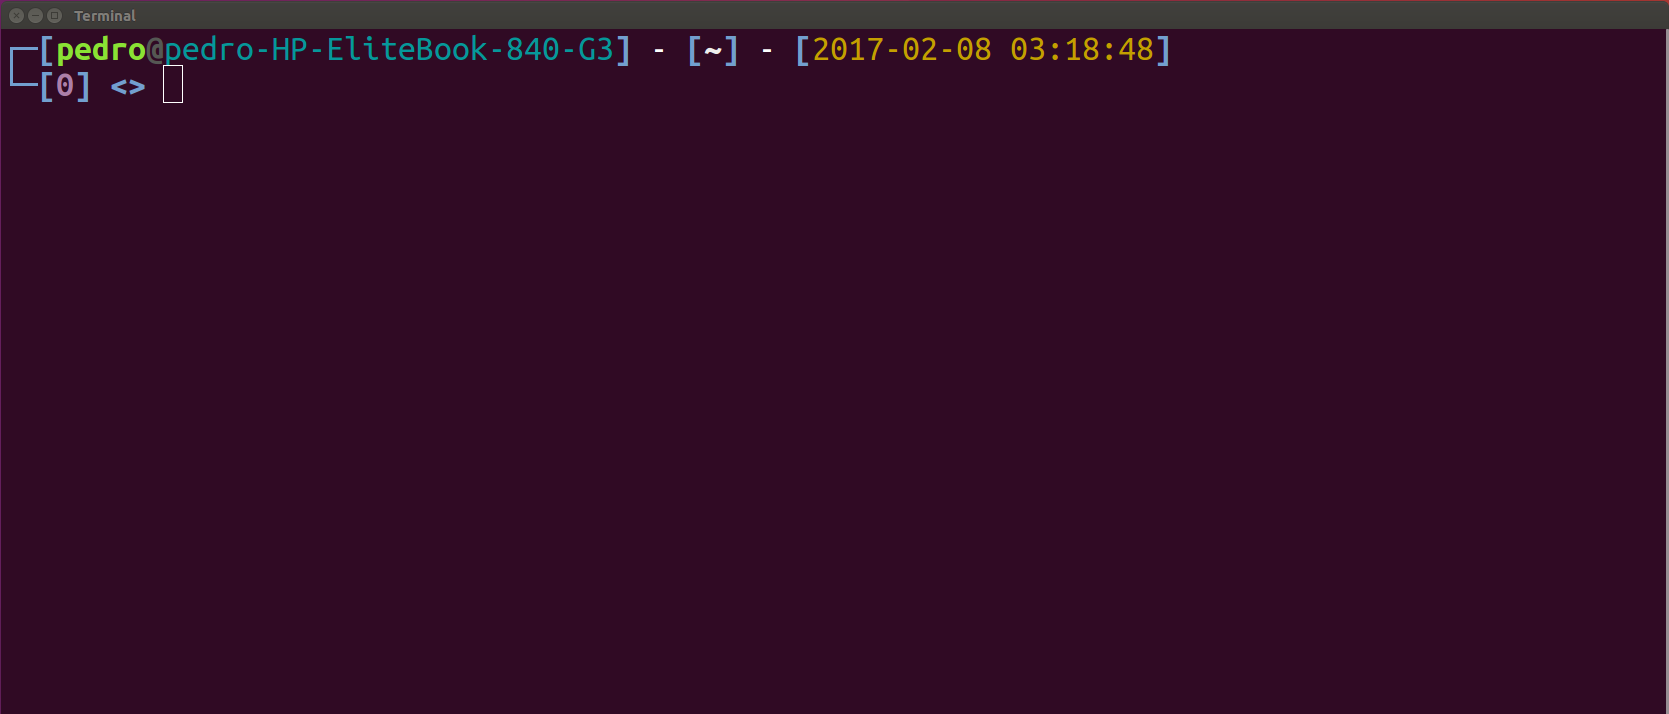
\includegraphics[width=9.5cm]{images/terminal_linux.png}
        \end{center}
	\begin{itemize}
		\item	on the terminal you can see the so-called Prompt
		\item	here you can control your PC/account or even
                 a remote server
	\end{itemize}
	
\end{frame}

%%%%%%%%%%%%%%%%%%%%%%%%%%%%%%%%%%%%%%%%%%%%%%%%%%%%%%%%%%%%%%%%%%%%%%%%%%%%%%%%%%%%%
\begin{frame}
	\frametitle{Files organization}
        \begin{center}
        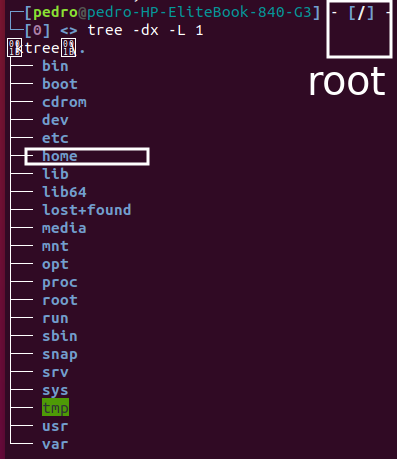
\includegraphics[width=7.5cm]{images/tree_root.png}
        \end{center}
\end{frame}
%%%%%%%%%%%%%%%%%%%%%%%%%%%%%%%%%%%%%%%%%%%%%%%%%%%%%%%%%%%%%%%%%%%%%%%%%%%%%%%%%%%%%
\begin{frame}
	\frametitle{Files organization}
        \begin{center}
        \includegraphics[width=10cm]{images/tree_organization.png}
        \end{center}
\end{frame}

%%%%%%%%%%%%%%%%%%%%%%%%%%%%%%%%%%%%%%%%%%%%%%%%%%%%%%%%%%%%%%%%%%%%%%%%%%%%%%%%%%%%%
\begin{frame}[fragile]
	\frametitle{ man}
        Manual pages. 
       
	\begin{itemize}
		\item \textbf{man command: man nano}
	\end{itemize}

{\tiny
	\begin{verbatim}
NANO(1)                     General Commands Manual                    NANO(1)

NAME
       nano - Nano's ANOther editor, an enhanced free Pico clone

SYNOPSIS
       nano [options] [[+line,column] file]...

DESCRIPTION
       nano  is  a small, free and friendly editor which aims to replace Pico,
       the default editor included in the non-free Pine package.   On  top  of
       copying  Pico's  look  and  feel, nano also implements some missing (or
       disabled by default) features in Pico, such as "search and replace" and
       "go to line and column number".
	\end{verbatim}
}
\end{frame}
%%%%%%%%%%%%%%%%%%%%%%%%%%%%%%%%%%%%%%%%%%%%%%%%%%%%%%%%%%%%%%%%%%%%%%%%%%%%%%%%%%%%%
\section{Navigating the File System}
\begin{frame}[fragile]
	\frametitle{}
\begin{center}
{\Huge
Navigating the File System
}
\end{center}

\end{frame}

%%%%%%%%%%%%%%%%%%%%%%%%%%%%%%%%%%%%%%%%%%%%%%%%%%%%%%%%%%%%%%%%%%%%%%%%%%%%%%%%%%%%%
\begin{frame}[fragile]
	\frametitle{ls}
List the content of a directory
{\scriptsize
	\begin{verbatim}
$ls
1CD9

$ls -l
total 24843644
drwxrwxr-x  2 pedro pedro        4096 nov  9 11:17 1CD9

$ls -la
total 24844368
drwxr-xr-x 44 pedro pedro        4096 feb 13 13:19 .
drwxr-xr-x  3 root  root         4096 sep 19 11:05 ..
drwxrwxr-x  2 pedro pedro        4096 nov  9 11:17 1CD9

$ls -lah
total 24G
drwxr-xr-x 44 pedro pedro 4,0K feb 13 13:25 .
drwxr-xr-x  3 root  root  4,0K sep 19 11:05 ..
drwxrwxr-x  2 pedro pedro 4,0K nov  9 11:17 1CD9
	\end{verbatim}
}

\end{frame}
%%%%%%%%%%%%%%%%%%%%%%%%%%%%%%%%%%%%%%%%%%%%%%%%%%%%%%%%%%%%%%%%%%%%%%%%%%%%%%%%%%%%%
\begin{frame}[fragile]
	\frametitle{ ls}
{\scriptsize
	\begin{verbatim}
$ls -laht
total 24G
drwxr-xr-x 44 pedro pedro 4,0K feb 13 13:29 .
-rw-------  1 pedro pedro 431K feb 13 13:29 .zsh_history
drwx------  6 pedro pedro 4,0K feb 13 13:28 Linux_Abisko_Kebne

$ls -lahrt
total 24G
-rw-r--r--  1 pedro pedro  655 sep 19 11:05 .profile
	\end{verbatim}
}

\end{frame}
%%%%%%%%%%%%%%%%%%%%%%%%%%%%%%%%%%%%%%%%%%%%%%%%%%%%%%%%%%%%%%%%%%%%%%%%%%%%%%%%%%%%%
\begin{frame}[fragile]
	\frametitle{ chmod}
Change permissions.

Useful cases:
	\begin{itemize}
        \item chmod Y+Z 
        \item Y=u,g,o 
        \item Z=r,w,x
	\end{itemize}
        
\end{frame}

%%%%%%%%%%%%%%%%%%%%%%%%%%%%%%%%%%%%%%%%%%%%%%%%%%%%%%%%%%%%%%%%%%%%%%%%%%%%%%%%%%%%%
\begin{frame}[fragile]
	\frametitle{ cd}
Change directory.

Useful cases:
	\begin{itemize}
        \item cd directory 

        move to "directory" 
        \item cd
 
         move to $\$HOME$ directory
        \item cd - 

        move to previous visited directory

        \item cd ..

        move to upper directory in the hierarchical tree

        \item pwd 
        prints out the local directory path
 
	\end{itemize}
        
\end{frame}

%%%%%%%%%%%%%%%%%%%%%%%%%%%%%%%%%%%%%%%%%%%%%%%%%%%%%%%%%%%%%%%%%%%%%%%%%%%%%%%%%%%%%
\begin{frame}
	\frametitle{ cp}
        Copy files.

Useful cases:
	\begin{itemize}
        \item cp text.txt directory/

        copy text.txt file to "directory" 
        \item cp -r test/ directory/ 
 
        copy the directory test into directory/. 

        cp overwrites existing files!

	\end{itemize}
        

\end{frame}


%%%%%%%%%%%%%%%%%%%%%%%%%%%%%%%%%%%%%%%%%%%%%%%%%%%%%%%%%%%%%%%%%%%%%%%%%%%%%%%%%%%%%
\begin{frame}
	\frametitle{ touch/mkdir}
        Create files.

Useful cases:
	\begin{itemize}
        \item touch text.txt

        creates text.txt file  
        \item mkdir test  
 
        creates the directory test 

	\end{itemize}

\end{frame}

%%%%%%%%%%%%%%%%%%%%%%%%%%%%%%%%%%%%%%%%%%%%%%%%%%%%%%%%%%%%%%%%%%%%%%%%%%%%%%%%%%%%%
\begin{frame}
	\frametitle{ rm}
        Remove files.

Useful cases:
	\begin{itemize}
        \item rm text.txt

        deletes text.txt file  
        \item rm -rf test/  
 
        deletes the directory test 

        deleted files cannot be recovered!

	\end{itemize}
        

\end{frame}

%%%%%%%%%%%%%%%%%%%%%%%%%%%%%%%%%%%%%%%%%%%%%%%%%%%%%%%%%%%%%%%%%%%%%%%%%%%%%%%%%%%%%
\begin{frame}
	\frametitle{Wild cards}

	\begin{itemize}
        \item ?

        it represents a single character

        \item *

        it represents a string of characters
 
        \item $\left[0-9\right], \left[A-B\right]$

        it represents a range of numbers or characters
	\end{itemize}
        

\end{frame}
%%%%%%%%%%%%%%%%%%%%%%%%%%%%%%%%%%%%%%%%%%%%%%%%%%%%%%%%%%%%%%%%%%%%%%%%%%%%%%%%%%%%%
\begin{frame}[fragile]
	\frametitle{Symbolic links}

also called soft links is a pointer file to other file/directory. One can create
a soft link with the $ln$ command: 
        
\begin{verbatim}
ln -s source.txt link

ls -l source.txt link 
lrwxrwxrwx 1 pedro pedro 14 sep  8 22:14 link -> source.txt
-rw-r--r-- 1 pedro pedro  0 sep  8 22:13 source.txt
\end{verbatim}


\end{frame}
%%%%%%%%%%%%%%%%%%%%%%%%%%%%%%%%%%%%%%%%%%%%%%%%%%%%%%%%%%%%%%%%%%%%%%%%%%%%%%%%%%%%%
\begin{frame}[fragile]
	\frametitle{Redirection}

       
we can change the standard input (keyboard)/output (screen) of Linux commands:
 

\begin{itemize}
   \item The operator $>$ redirects the output of some command 

   $ls > test.dat$

   in this case to the file test.dat

   \item The operator $>>$ concatenate the output of some command to the content 
   of a file:

   $ls >> test.dat$

   \item The operator $<$ changes the standard input

   \item The operator $2>$ redirects the standard error:

   $exec 2>error.log$

   \item The operator $2>\&1$, redirects both standard output and error:
   $exec > logfile  2>\&1$
\end{itemize}


\end{frame}
%%%%%%%%%%%%%%%%%%%%%%%%%%%%%%%%%%%%%%%%%%%%%%%%%%%%%%%%%%%%%%%%%%%%%%%%%%%%%%%%%%%%%
\begin{frame}[fragile]
	\frametitle{Pipes}
	\begin{itemize}
         \item  One can use the output of some command as the input for another command:
	\end{itemize}

\begin{verbatim}
grep 'string' file.txt | wc 
grep 'string' file.txt > file.out
grep 'string' file.txt >> file.out
\end{verbatim}

\end{frame}
%%%%%%%%%%%%%%%%%%%%%%%%%%%%%%%%%%%%%%%%%%%%%%%%%%%%%%%%%%%%%%%%%%%%%%%%%%%%%%%%%%%%%
\begin{frame}[fragile]
	\frametitle{Exporting variables}

\begin{itemize}
   \item some programs or libraries require environment variables to work
   \item they allow the program to follow different schemes without being re-compiled
   \item some variables such as $\$HOME$ are intrinsic to Linux OS
   \item we need to export the variables for further use:

\begin{verbatim}
$export NUMBER_OF_THREADS=6
\end{verbatim}
\end{itemize}

\end{frame}
%%%%%%%%%%%%%%%%%%%%%%%%%%%%%%%%%%%%%%%%%%%%%%%%%%%%%%%%%%%%%%%%%%%%%%%%%%%%%%%%%%%%%
\begin{frame}
	\frametitle{Editing files}
        \begin{center}
        \includegraphics[width=10cm]{images/nano.png}
        \end{center}
\end{frame}

%%%%%%%%%%%%%%%%%%%%%%%%%%%%%%%%%%%%%%%%%%%%%%%%%%%%%%%%%%%%%%%%%%%%%%%%%%%%%%%%%%%%%
\section{Data Handling}
\begin{frame}[fragile]
	\frametitle{}
\begin{center}
{\Huge
Data Handling
}
\end{center}

\end{frame}


%%%%%%%%%%%%%%%%%%%%%%%%%%%%%%%%%%%%%%%%%%%%%%%%%%%%%%%%%%%%%%%%%%%%%%%%%%%%%%%%%%%%%
\begin{frame}[fragile]
	\frametitle{Compress/decompress files}

Compressing files:

\begin{verbatim}
$gzip file     --->  file.gz
\end{verbatim}

Decompressing files:

\begin{verbatim}
$gunzip file.gz
\end{verbatim}

\end{frame}

%%%%%%%%%%%%%%%%%%%%%%%%%%%%%%%%%%%%%%%%%%%%%%%%%%%%%%%%%%%%%%%%%%%%%%%%%%%%%%%%%%%%%

\begin{frame}[fragile]
	\frametitle{Generating archives}

Generate tar-ball:

\begin{verbatim}
$tar -cvf directory.tar directory 
\end{verbatim}

Opening tar-ball:

\begin{verbatim}
$tar -xvf directory.tar
\end{verbatim}

\end{frame}


%%%%%%%%%%%%%%%%%%%%%%%%%%%%%%%%%%%%%%%%%%%%%%%%%%%%%%%%%%%%%%%%%%%%%%%%%%%%%%%%%%%%%
\begin{frame}
	\frametitle{ ssh}
Command for connecting to a remote computer.

Useful cases:
	\begin{itemize}
         \item ssh username@abisko.hpc2n.umu.se

         connecting to abisko machine

         \item ssh -Xl username abisko.hpc2n.umu.se

        if you want to enable graphical display.

	\end{itemize}
\end{frame}

%%%%%%%%%%%%%%%%%%%%%%%%%%%%%%%%%%%%%%%%%%%%%%%%%%%%%%%%%%%%%%%%%%%%%%%%%%%%%%%%%%%%%
\begin{frame}[fragile]
	\frametitle{ sftp (scp)}

Protocol for data transfer.
\begin{verbatim}
$sftp username@abisko.hpc2n.umu.se

$get file

$put file

\end{verbatim}
\end{frame}

%%%%%%%%%%%%%%%%%%%%%%%%%%%%%%%%%%%%%%%%%%%%%%%%%%%%%%%%%%%%%%%%%%%%%%%%%%%%%%%%%%%%%
\begin{frame}[fragile]
	\frametitle{ rsync}

Protocol for synchronizing data.
\begin{verbatim}
rsync source target

rsync -az user@kebne.hpc2n.umu.se:/home/proj/ proj/
\end{verbatim}
\end{frame}


\section{Finding Patterns}
%%%%%%%%%%%%%%%%%%%%%%%%%%%%%%%%%%%%%%%%%%%%%%%%%%%%%%%%%%%%%%%%%%%%%%%%%%%%%%%%%%%%%
\begin{frame}[fragile]
	\frametitle{}
\begin{center}
{\Huge
Finding patterns
}
\end{center}

\end{frame}

%%%%%%%%%%%%%%%%%%%%%%%%%%%%%%%%%%%%%%%%%%%%%%%%%%%%%%%%%%%%%%%%%%%%%%%%%%%%%%%%%%%%%
\begin{frame}
	\frametitle{ grep}
      This command searches for patterns in text files.

Useful cases:
	\begin{itemize}
        \item grep 'word' file

        it searches for pattern 'word' in file

        \item grep -rine 'word' home

        pattern word is searched recursively in the directory  $/home$
 
	\end{itemize}

\end{frame}

%%%%%%%%%%%%%%%%%%%%%%%%%%%%%%%%%%%%%%%%%%%%%%%%%%%%%%%%%%%%%%%%%%%%%%%%%%%%%%%%%%%%%
\begin{frame}
	\frametitle{ awk}
This command finds patterns in a file and can perform arithmetic/string operations.

Useful cases:
	\begin{itemize}
        \item awk '/gold/ $\{print  \$1 \} $' file

        \item it searches for pattern 'gold' in file and prints out the first column 

	\end{itemize}

\end{frame}

%%%%%%%%%%%%%%%%%%%%%%%%%%%%%%%%%%%%%%%%%%%%%%%%%%%%%%%%%%%%%%%%%%%%%%%%%%%%%%%%%%%%%
\section{Scripting}
\begin{frame}[fragile]
	\frametitle{}
\begin{center}
{\Huge
Scripting
}
\end{center}

\end{frame}


\begin{frame}
	\frametitle{Scripting}

\begin{itemize}
\item allows to perform complex tasks without user intervention
\item all Linux commands can be used in a script including wild cards

\end{itemize}

\end{frame}
%%%%%%%%%%%%%%%%%%%%%%%%%%%%%%%%%%%%%%%%%%%%%%%%%%%%%%%%%%%%%%%%%%%%%%%%%%%%%%%%%%%%%

\begin{frame}[fragile]
	\frametitle{Scripting}

\begin{block}{analysis.sh}
\begin{verbatim}
#!/bin/bash

grep 'ABCD' file.pdb >  file_filtered.pdb 

program < file_filtered.pdb > output.dat

\end{verbatim}
\end{block}

execute script with ./analysis.sh

\end{frame}
%%%%%%%%%%%%%%%%%%%%%%%%%%%%%%%%%%%%%%%%%%%%%%%%%%%%%%%%%%%%%%%%%%%%%%%%%%%%%%%%%%%%%

\begin{frame}[fragile]
	\frametitle{Scripting}

\begin{verbatim}
$ls -lah
total 24G
drwxrwxr-x  2 pedro pedro 4,0K nov  9 11:17 1CD9
\end{verbatim}

\begin{itemize}
\item permissions are set of "user", "group", or "others"
\item we can change permissions with chmod command
\end{itemize}

For instance, 

\begin{verbatim}
$chmod u+x analysis.sh

$execute script with ./analysis.sh
\end{verbatim}

\end{frame}

%%%%%%%%%%%%%%%%%%%%%%%%%%%%%%%%%%%%%%%%%%%%%%%%%%%%%%%%%%%%%%%%%%%%%%%%%%%%%%%%%%%%%

\section{More advanced topics}

\begin{frame}[fragile]
	\frametitle{Working with the Prompt}

\begin{itemize}
\item ctrl+a:	Go to the beginning of the line
\item ctrl+e:	Go to the end of the line
\item ctrl+l:   Clean the terminal
\end{itemize}

\end{frame}

%%%%%%%%%%%%%%%%%%%%%%%%%%%%%%%%%%%%%%%%%%%%%%%%%%%%%%%%%%%%%%%%%%%%%%%%%%%%%%%%%%%%%
\begin{frame}[fragile]
	\frametitle{Configuring .bashrc file}

Exploring the history:

by typing "ctrl+r" you will be prompted to introduce text which bash 
will use to make a search in the list of commands you have typed previously.
That list is saved in the .bash\_history file in your home directory.  

One can control the behavior of the history file by setting environment variables
in the .bashrc file as follows:

\begin{verbatim}
export HISTCONTROL=erasedups
export HISTSIZE=100000
export HISTFILESIZE=100000
shopt -s histappend
\end{verbatim}


\end{frame}
%%%%%%%%%%%%%%%%%%%%%%%%%%%%%%%%%%%%%%%%%%%%%%%%%%%%%%%%%%%%%%%%%%%%%%%%%%%%%%%%%%%%%
\begin{frame}[fragile]
	\frametitle{Configuring .bashrc file}

Using aliases:

if you need to type a long command several times, you may add it as an alias in 
your .bashrc file:

\begin{verbatim}
alias ldir='ls -lahrt | egrep "^d"'
\end{verbatim}

\end{frame}
%%%%%%%%%%%%%%%%%%%%%%%%%%%%%%%%%%%%%%%%%%%%%%%%%%%%%%%%%%%%%%%%%%%%%%%%%%%%%%%%%%%%%
\begin{frame}[fragile]
	\frametitle{Specific commands on our cluster}

\begin{itemize}
\item projinfo: information of the usage of the project resources
\item squeue -a -u username: status of the jobs for username
\item sbatch script.sh: for job submission
\item scancel jobid: for cancelling a job
\item quota: information of the /home and /pfs disk usage
\end{itemize}

\end{frame}
%%%%%%%%%%%%%%%%%%%%%%%%%%%%%%%%%%%%%%%%%%%%%%%%%%%%%%%%%%%%%%%%%%%%%%%%%%%%%%%%%%%%%

\begin{frame}
	\frametitle{Linux Cheat Sheet}

\begin{itemize}
\item https://www.hpc2n.umu.se/documentation/guides/linux-cheat-sheet
\end{itemize}

\end{frame}
